\documentclass[a4paper, 12pt]{article}
\usepackage{comment} % enables the use of multi-line comments (\ifx \fi)
\usepackage{graphicx}
\usepackage{fullpage} % changes the margin
\usepackage{listings}
\usepackage{xparse}
\usepackage{xcolor}
\usepackage{minted}
\usepackage{amsmath}
\usepackage{varwidth}
\usepackage{tikz}

\usetikzlibrary{shapes,arrows,automata}

\tikzstyle{block} = [draw, fill=blue!20, rectangle, 
    minimum height=3em, minimum width=6em]
\tikzstyle{sum} = [draw, fill=blue!20, circle, node distance=1cm]
\tikzstyle{input} = [coordinate]
\tikzstyle{output} = [coordinate]
\tikzstyle{pinstyle} = [pin edge={to-,thin,black}]

\NewDocumentCommand{\codeword}{v}{%
\texttt{\textcolor{blue}{#1}}%
}

\newcommand{\block}[1]{%
  \begingroup
  \setlength{\fboxsep}{0pt}%
  \vrule width0pt height \blockdim
  \ooalign{%
    \framebox[\blockdim]{\rule{0pt}{\blockdim}}\cr
    \hidewidth\raisebox{0.5\dimexpr\blockdim-\height}{\raisebox{\depth}{#1}}\hidewidth\cr
  }%
  \endgroup
}
\newcommand{\joinblocks}{\unskip\kern-\fboxrule\ignorespaces}
\newenvironment{blocks}[1][1cm]
 {\begin{varwidth}{\textwidth}\setlength{\blockdim}{#1}\makeblocks}
 {\end{varwidth}}
\newcommand{\makeblocks}{%
  \begingroup\lccode`~=`&\lowercase{\endgroup\let~}\joinblocks
  \catcode`\&=\active
  \baselineskip=0pt
  \lineskiplimit=\maxdimen
  \lineskip=0pt
  \centering
}
\newlength{\blockdim}

\begin{document}
% Header
\noindent
\LARGE\textbf{Intrastellar} \hfill \\
\newline
\large\textbf{Final Report} \hfill \textbf{Zach Schuermann} \\
\normalsize ECE 4273-001 \hfill 112944063 \\
Dr. Erik Petrich \hfill Date: 05/03/19 

\section*{Project Objectives}
The goal for this project was to create a retro video game using the LPC1769 and supporting hardware. I elected to create a Galaga-like game implemented on an LPC1769 with a Playstation 2 controller for user input/control and a 480x800 LCD display. The gameplay will be in real-time with the goal of destroying circular asteroids as they advance towards your spacecraft. In general, there are three main subsystems: display, controller input, and sound. The sound subsystem was unnecessary for the completion of the project objectives, and as such was omitted from the game, instead the EEPROM was used. Thus the subsystems slightly changed from the preliminary design report, and the three systems are now: display, controller, and EEPROM. The game continuously polls for controller input, runs the game logic, and renders the screen (via the display driver). 

\section*{User Guide}
Interaction with the game is relatively simple. In its current implementation, all user interaction is facilitated with the 'X' button and the left and right bottom bumpers (triggers) on the Playstation controller. A start screen appears on power up (after 9V is applied for the power rail corresponding to the display and USB power is provided to the LPC1769) displaying the current high score. After pressing 'X', the game begins and the user must destroy the asteroids by moving the ship with the triggers and shooting bullets with the 'X' button. You are awarded 100 points each time you destroy an asteroid. The game continues until you have no lives left. You begin with three lives and lose one for each asteroid that makes it past your ship. Upon reaching the end of the game, you will be shown your score and given the option to play again! Figure \ref{fig:screen} provides a screenshot showing gameplay.

\begin{figure}[h!]
  \centering
  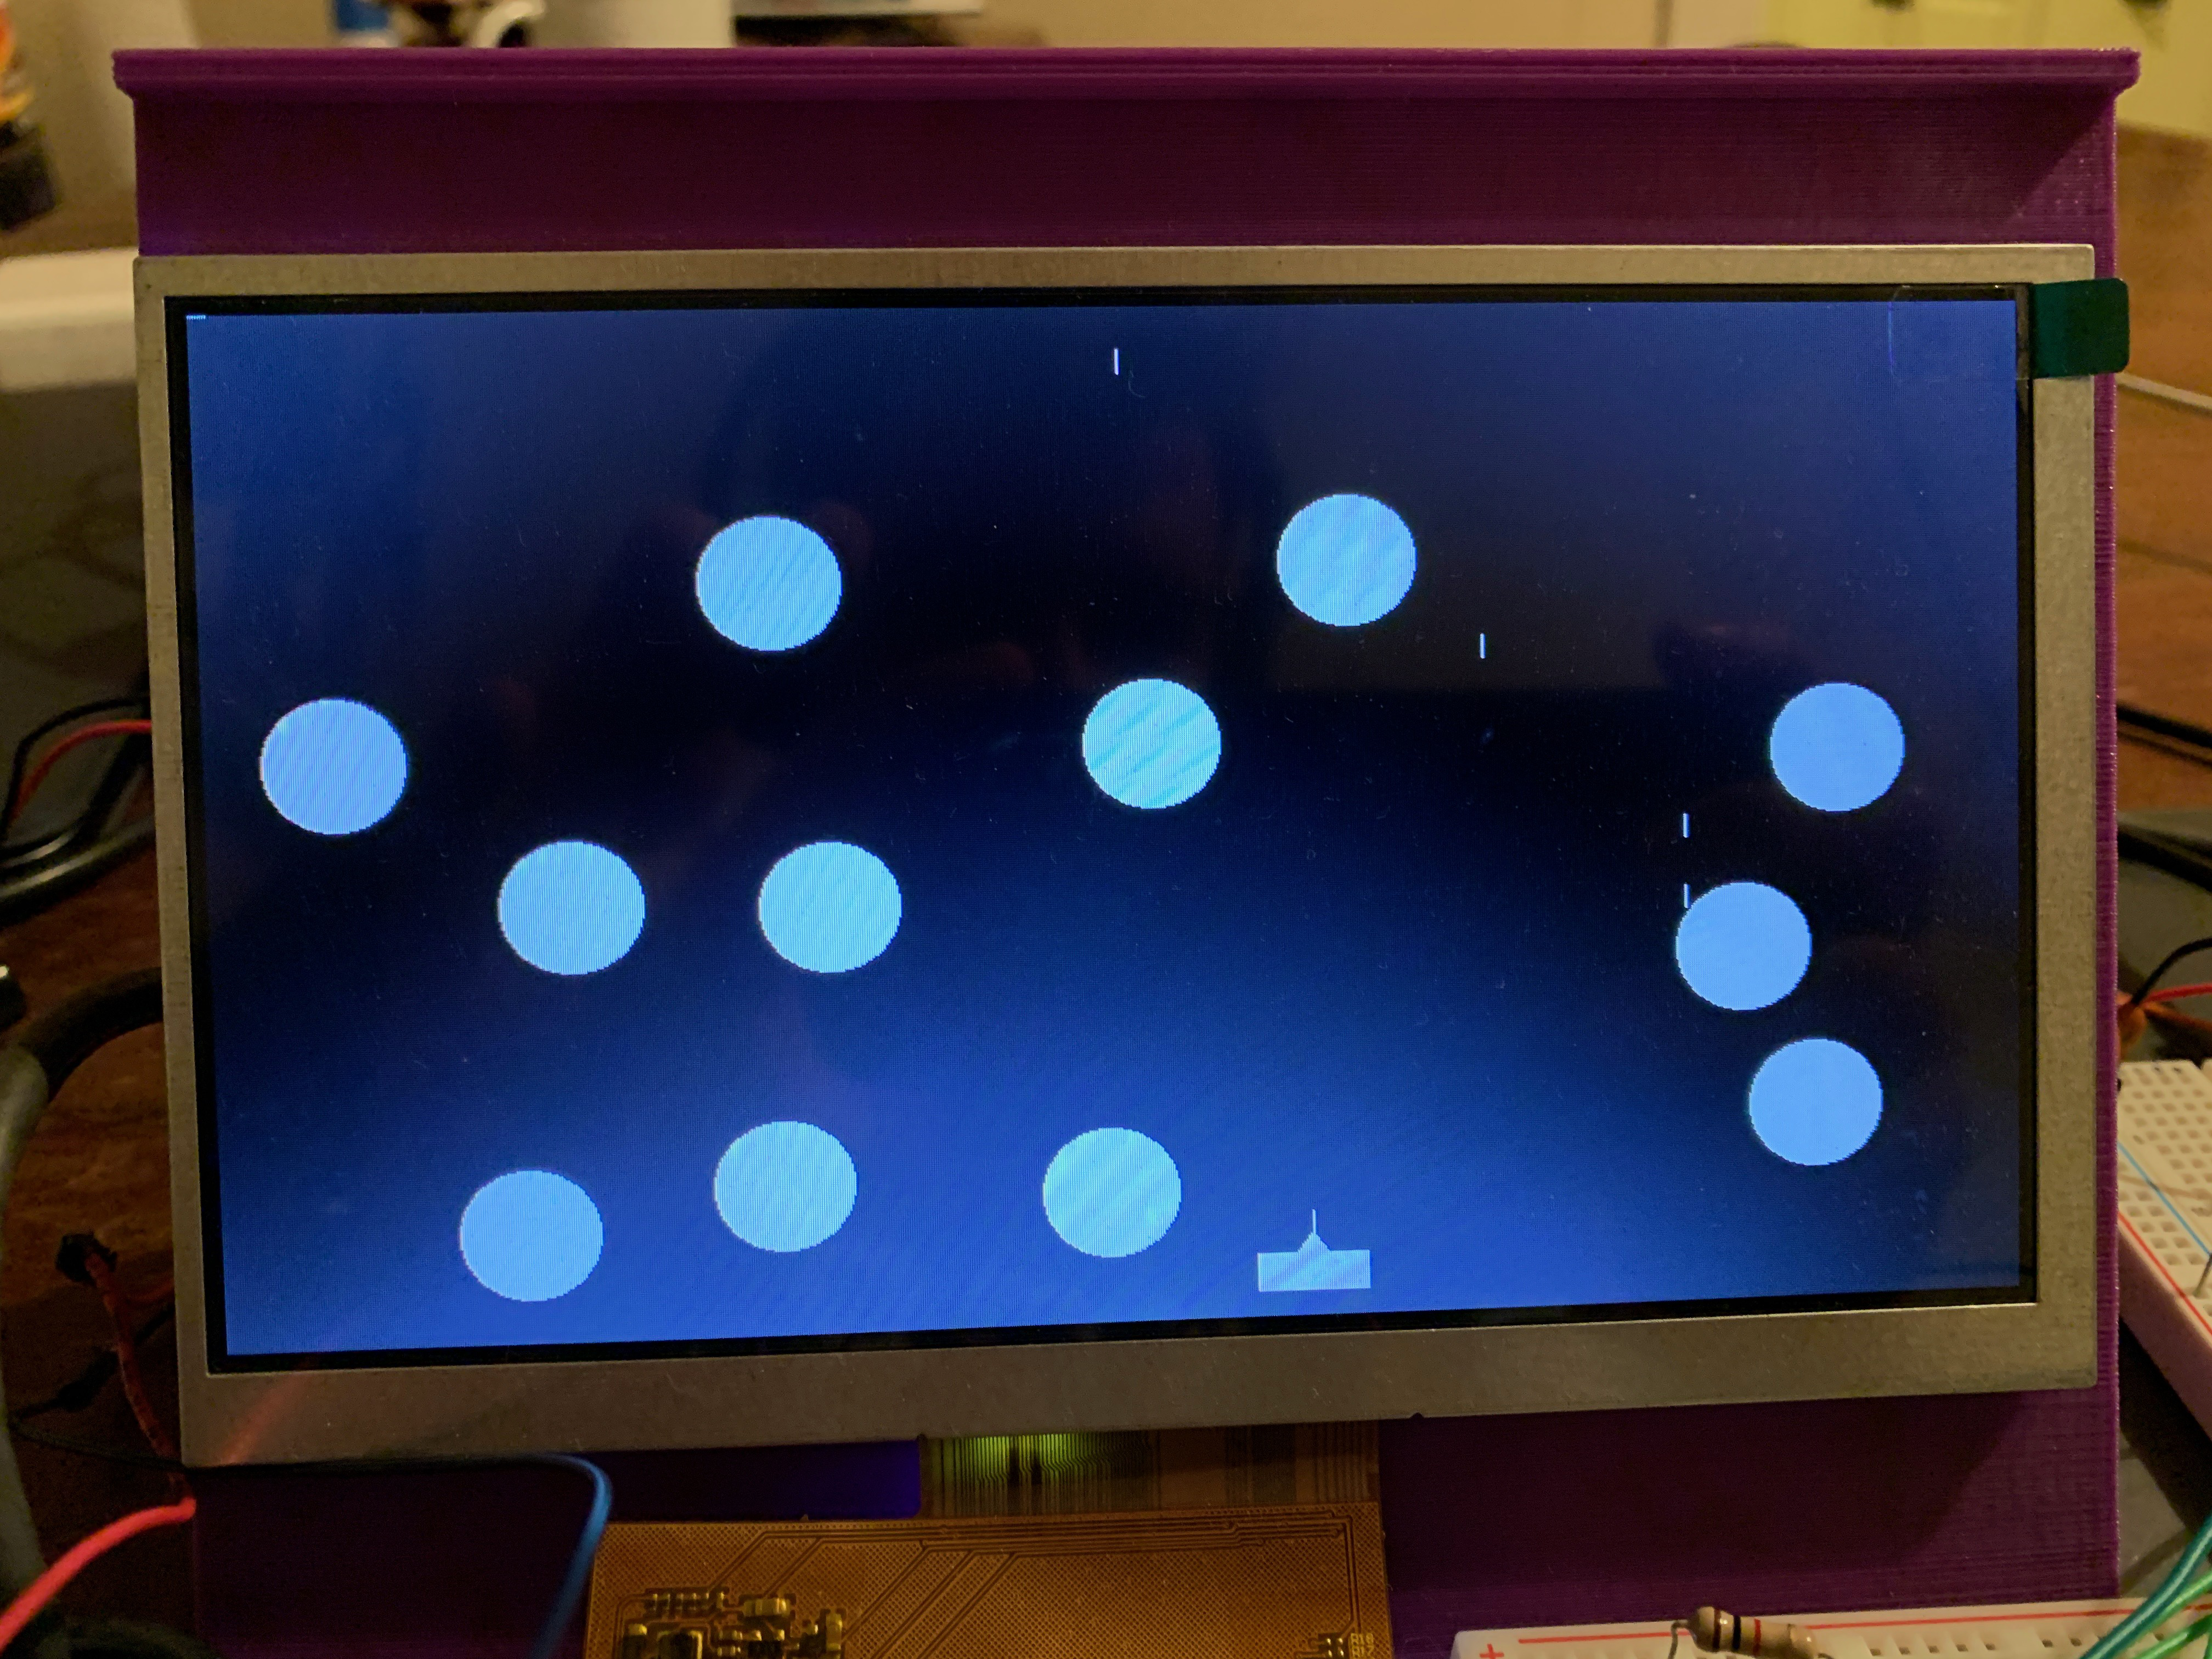
\includegraphics[scale=.1]{screen.png}
  \caption{Gameplay Screenshot}
  \label{fig:screen}
\end{figure}

\section*{Project Design}
The final construction of the project is shown in Figure \ref{fig:pic}. The project implements the following features:

\begin{center}
  {\footnotesize
  \begin{tabular}{ |c|c|c|c| }
    \hline
    \textbf{Component} & \textbf{Description} & \textbf{Points} & \textbf{Completed} \\
    \hline
    \hline
    Game Type & Animated real-time game (objects continuously in motion) & 2 & YES\\
    \hline
    Display & Use a graphical LCD for output  & 2 & YES\\
    \hline
    Input & Use a game controller with a serial interface (Playstation 2) & 0.5 & YES\\ 
    \hline
    Sound & Use D-to-A to generate a sine wave based sound effect  & 1 & NO\\
    \hline
    Other & Use non-volatile memory (EEPROM  to retain high score table) & 0.5 & YES\\ 
    \hline
    Total & & 5 & \\ 
    \hline
  \end{tabular}
  }
\end{center}

\begin{figure}[h!]
  \centering
  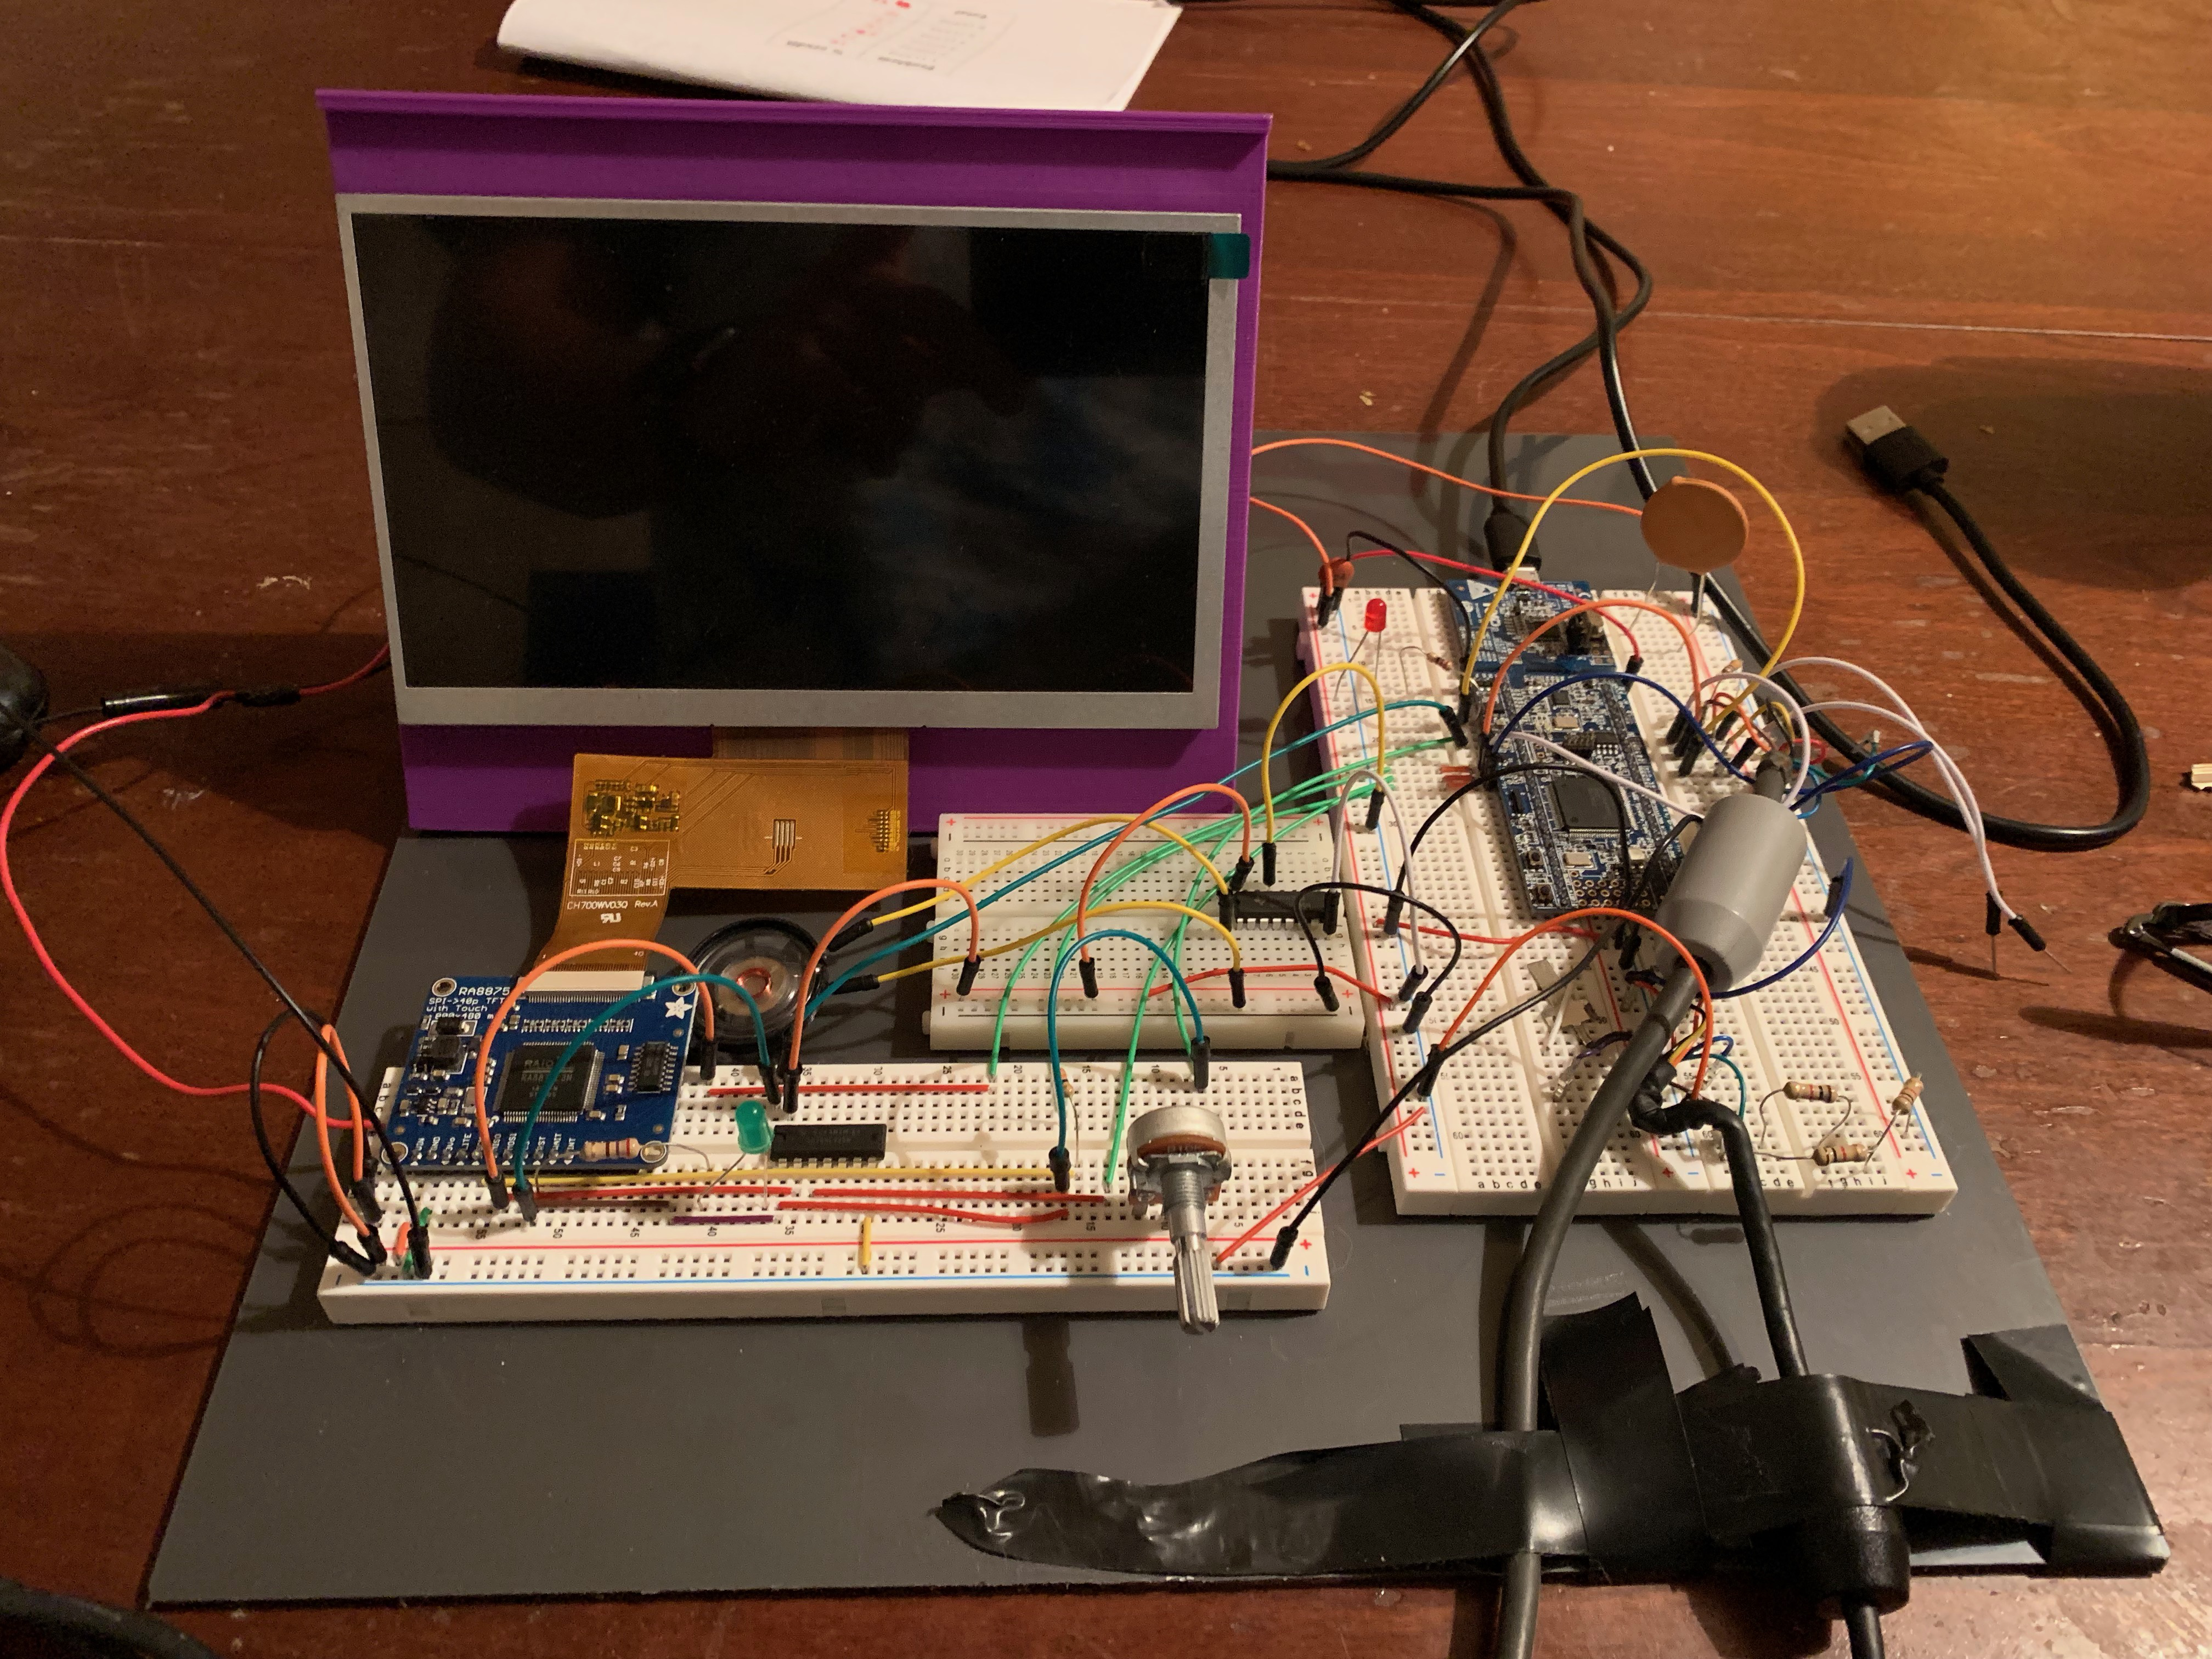
\includegraphics[scale=.1]{pic.png}
  \caption{Final Implementation}
  \label{fig:pic}
\end{figure}

\subsection*{Display Sub-System}
The display subsystem relies on an Adafruit 40-pin LCD 480x800 7" display. In order to effectively communicate with such a large display, an intermediate processor is utilized. The Adafruit RA8875 Display Driver Board was selected as a sufficient intermediary. The board has 768 kB of memory to store the entire frame buffer, and is easily changed via SPI. Furthermore, there are a number of hardware-accelerated functions for drawing specific shapes. This system operates on a 2 MHz SPI clock in order to pass information quickly between the driver and the microcontroller.  

\subsection*{Controller Sub-System}
The Playstation 2 (PS2) controller will act as the means for the user to control the game. The PS2 controller uses a serial protocol which is essentially SPI. In order to communicate, the clock rate will require decreasing to about 250 kHz. To facilitate communication for both the controller and the display, a common clock division is used at the peripheral interface. The clock signal is then further divided to produce either the 250 kHz clock or the 2 MHz clock.

\subsection*{EEPROM}
Lastly, the design relies on the onboard EEPROM to save the high score to a location which will not clear on power cycling. This system is already implemented on the LPCXpresso development board via the I2C subsystem. 

\section*{Hardware Design}

\begin{figure}[h!]
  \centering
  \includegraphics[scale=.18]{schematic.png}
  \caption{Preliminary Hardware Schematic}
  \label{fig:schematic}
\end{figure}

The schematic in Figure \ref{fig:schematic} illustrates the hardware design for the project. 

\section*{Software Design}
The software design includes the adaptation of the Adafruit RA8875 library for our microcontroller, game logic, and controller communication. The many subsystems referenced above require configuring through software. Furthermore, the processor is clocked at 96 MHz in order to provide for sufficient speed for SPI communication as well as executing game logic and rendering quickly. Aside from configuration and communication, the software enters a game loop which continuously polls the controller for input, runs the game logic, and renders the output. In order to hold the state of the game, a global \codeword{game} struct is used. The entire architecture for the game is succinctly described as follows: the game struct is initialized and subsequently modified with the game logic and polling the controller state. The struct is then rendered to the display. The game loop implements all of the aforementioned tasks. In order to maintain constant velocity for the bullets and asteroids, their locations are changed in the system tick handler interrupt to ensure constant velocity.
The game logic essentially just checks for lives lost and bullet/asteroid collisions. The logic implemented also checks for bullets reaching the top end of the screen and removing them from the game. Upon a collision, points are awarded and the bullet and asteroid are removed from the struct. In the current implementation, memory is statically allocated to support up to 50 asteroids/bullets at once. 

\clearpage

\section*{Appendix: Oscilloscope Screen Captures}
\begin{figure}[h!]
  \centering
  \includegraphics[scale=.5]{controller.png}
  \caption{Controller SPI interaction sequence}
  \label{fig:sce}
\end{figure}
\begin{figure}[h!]
  \centering
  \includegraphics[scale=.5]{init-display.png}
  \caption{Display initialization sequence}
  \label{fig:stic}
\end{figure}
\begin{figure}[h!]
  \centering
  \includegraphics[scale=.5]{full-display.png}
  \caption{Full display interaction sequence}
  \label{fig:shmatic}
\end{figure}


\clearpage
\section*{Appendix: Source}
\section*{intrastellar.c}
\inputminted{c}{src/intrastellar.c}
\clearpage
\section*{eeprom.c}
\inputminted{c}{src/eeprom.c}
\clearpage
\section*{lcd.c}
\inputminted{c}{src/lcd.c}
\clearpage
\section*{ps2.c}
\inputminted{c}{src/ps2.c}
\clearpage
\section*{intrastellar.h}
\inputminted{c}{inc/intrastellar.h}
\clearpage
\section*{eeprom.h}
\inputminted{c}{inc/eeprom.h}
\clearpage
\section*{lcd.h}
\inputminted{c}{inc/lcd.h}
\clearpage
\section*{ps2.h}
\inputminted{c}{inc/ps2.h}

\end{document}
